% !TEX TS-program = xelatex
% !BIB TS-program = bibtex
\documentclass[12pt,letterpaper]{article}
\usepackage{style/dsc180reportstyle}
\definecolor{RoyalBlue}{RGB}{65,105,225}
\definecolor{BrickRed}{RGB}{203,65,84}
\renewcommand{\_}{\textunderscore\allowbreak}
\emergencystretch=2em
\usepackage{colortbl}
\definecolor{scorehi}{HTML}{C8E6C9}
\definecolor{scoremid}{HTML}{FFF9C4}
\definecolor{scorelo}{HTML}{FFCDD2}
\definecolor{scorena}{HTML}{EEEEEE}
\definecolor{ForestGreen}{RGB}{34,139,34}
\definecolor{Goldenrod}{RGB}{218,165,32}

\title{Training-based versus training-free \\ differential privacy for data synthesis}

\author{Mehak Kapur \\
  {\tt mekapur@ucsd.edu} \\\And
  Hana Tjendrawasi  \\
  {\tt htjendrawasi@ucsd.edu} \\\And
  Jason Tran \\
  {\tt jat037@ucsd.edu} \\\And
  Phuc Tran \\
  {\tt pct001@ucsd.edu} \\\And
  Yu-Xiang Wang \\
  {\tt yuxiangw@ucsd.edu} \\}

\begin{document}
\maketitle

\begin{abstract}
Differentially private synthetic data generation promises to resolve the tension between data utility and individual privacy, enabling the release of datasets that preserve the statistical properties analysts need while bounding what any adversary can learn about a single record. Two paradigms have emerged to fulfill this promise. Training-based methods inject calibrated noise during model optimization, coupling privacy to the learning process itself. Training-free methods instead leverage foundation models through black-box API access, achieving privacy through selection mechanisms that never touch the model's parameters. Both have demonstrated success on image and text benchmarks, yet their behavior on realistic, multi-table relational data remains largely unexplored. We investigate both approaches on Intel's Driver and Client Applications (DCA) telemetry corpus, evaluating against a benchmark of 21 analytical SQL queries representative of production business intelligence workloads.
\end{abstract}

\begin{center}
Code: \url{https://github.com/jktrns/DSC180B-Q2}
\end{center}

\clearpage
\maketoc
\clearpage

\section{Introduction}

\subsection{Motivation}

Organizations routinely collect detailed telemetry from their products to drive business decisions. Engineers use it to diagnose failures, product teams analyze usage trends, and analysts extract insights that shape product roadmaps. The same granularity that makes telemetry valuable also makes it sensitive. Browsing patterns, work schedules, and device fingerprints can re-identify specific individuals even after conventional anonymization.

Privacy regulations such as GDPR and CCPA, along with institutional policies, increasingly restrict how such data can be stored, shared, and analyzed. The resulting tension between data utility and privacy protection motivates the development of \textit{synthetic data generation}, producing artificial datasets that preserve the statistical properties necessary for analysis while providing formal guarantees that no individual's information can be recovered.

Two paradigms have emerged for generating synthetic data with rigorous privacy guarantees. \textit{Training-based methods} optimize generative models under constraints that bound individual influence, adding calibrated noise during the training process. \textit{Training-free methods} leverage pre-trained foundation models through black-box API access, achieving privacy through carefully designed selection mechanisms rather than private optimization. Both approaches have demonstrated success in isolation on image and text benchmarks, yet no comprehensive comparison exists under controlled experimental conditions with realistic analytical workloads on multi-table relational data.

This project provides that comparison. We implement both paradigms on Intel's Driver and Client Applications (DCA) telemetry corpus and evaluate them against a benchmark of 21 SQL queries representative of production analytics, measuring which approach better preserves query fidelity under equivalent privacy budgets.

\subsection{Prior work}

Differential privacy, introduced by \citet{dwork2014algorithmic}, provides the foundational framework for our privacy guarantees. A randomized mechanism $\mathcal{M}$ is $(\varepsilon, \delta)$-differentially private if for all neighboring databases $D, D'$ differing by one record and all measurable output sets $S$:
\begin{equation}
    \Pr[\mathcal{M}(D) \in S] \leq e^{\varepsilon} \Pr[\mathcal{M}(D') \in S] + \delta.
\end{equation}
The parameter $\varepsilon$ controls the privacy-utility tradeoff. Smaller values confer stronger privacy at the cost of noisier outputs. The slack $\delta$ permits rare violations and must remain negligible relative to the database size. The work established key mechanisms (Laplace, Gaussian, exponential) for releasing numeric queries, along with composition theorems demonstrating that privacy loss accumulates across multiple analyses.

\citet{abadi2016deep} extended differential privacy to deep learning through DP-SGD. Standard gradient descent leaks information through the unbounded influence any single training example can exert on model parameters. DP-SGD bounds this influence by clipping each per-sample gradient to a fixed $\ell_2$ norm and injecting calibrated Gaussian noise to mask individual contributions. The accompanying \textit{moments accountant} yields substantially tighter privacy bounds than naive composition, enabling practical deep learning under modest privacy budgets.

\citet{ghalebikesabi2023differentially} demonstrated that fine-tuning diffusion models with DP-SGD generates synthetic images of reasonable quality, though their approach requires substantial privacy budgets ($\varepsilon \approx 32$ for CIFAR-10). This motivates the search for methods that achieve comparable fidelity at lower $\varepsilon$.

\citet{lin2025differentiallyprivatesyntheticdata} introduced Private Evolution (PE), a fundamentally different paradigm that avoids model training entirely. PE operates through black-box API access to pre-trained foundation models, iteratively evolving synthetic samples by computing differentially private nearest-neighbor histograms. Each private data point votes for its nearest synthetic candidate; Gaussian noise is added to the vote histogram, and candidates are resampled according to the noisy distribution. PE achieved FID $\leq 7.9$ at $\varepsilon = 0.67$ on CIFAR-10, a substantial improvement over DP-Diffusion in both privacy cost and output quality. The privacy analysis is straightforward. Each iteration releases one Gaussian mechanism, and $T$ iterations compose to a single mechanism with noise multiplier $\sigma / \sqrt{T}$.

\citet{xie2024differentiallyprivatesyntheticdata} extended PE to text through Aug-PE, introducing fill-in-the-blanks variation, adaptive text lengths, and rank-based selection. Aug-PE with GPT-3.5 outperformed DP-finetuning baselines at the same privacy budget while running 12--66$\times$ faster.

\citet{swanberg2025apiaccessllmsuseful} adapted PE for tabular data using a workload-aware distance function that measures proximity in terms of query-relevant predicates rather than raw feature similarity. Their central finding is negative. API access to large language models does not yet improve differentially private tabular synthesis beyond established marginal-based baselines such as MST and JAM. This result informs our expectations for applying PE to the DCA telemetry corpus.

\newpage

\section{Data and problem statement}

\subsection{Intel DCA telemetry data}

Our investigation uses the Intel Driver and Client Applications (DCA) telemetry dataset, a large-scale collection of system-level signals from Windows client machines. The full corpus comprises approximately 115 tables in the \texttt{university\_prod} schema (9.1~TB total), organized around a globally unique identifier (\texttt{guid}) assigned to each client system. Raw event tables record per-interval measurements (hourly or daily) across power, thermal, network, application, and browsing domains. Individual tables range from tens of millions to billions of rows.

The 24 benchmark queries do not reference the raw event tables directly. They reference a \texttt{reporting} schema of pre-aggregated views that Intel analysts built on top of the raw data. These reporting tables aggregate per-event measurements to per-\texttt{guid} summaries (or per-\texttt{guid}-per-day, depending on the table). Since the reporting views are not distributed with the raw data, we reconstruct them from the raw tables using DuckDB aggregation scripts that follow Intel's documented ETL logic.

We work with a sample of the full corpus. Each raw table in the repository is split into multiple partition files of varying size, and we download a single partition per table (the first available file, typically between 1 and 5~GiB). Several tables are supplemented or replaced entirely by pre-aggregated files from a December 2024 update that Intel added to the repository. The \texttt{system\_sysinfo\_unique\_normalized} anchor table is downloaded in full (1{,}000{,}000 \texttt{guid}s). All event tables are filtered to \texttt{guid}s present in this anchor, ensuring a coherent sample. Total data on disk is approximately 20.7~GiB.

Table~\ref{tab:reporting-tables} lists the 19 reporting tables we construct, organized by category. The \texttt{guid} coverage column reports how many of the 1{,}000{,}000 anchor \texttt{guid}s have at least one nonzero entry in each table. Coverage varies by two orders of magnitude. The web browsing pivot table covers 512{,}077 \texttt{guid}s (51.2\%), while the PSYS RAP power metric covers only 816 (0.08\%). This heterogeneous coverage is a defining characteristic of the dataset and, as we show in Section~4, a primary source of difficulty for synthesis.

\begin{footnotesize}
\begin{longtable}{>{\raggedright\arraybackslash}p{0.21\linewidth}>{\raggedright\arraybackslash}p{0.14\linewidth}>{\raggedright\arraybackslash}p{0.24\linewidth}>{\raggedright\arraybackslash}p{0.12\linewidth}>{\raggedright\arraybackslash}p{0.11\linewidth}}
\caption{The 19 reporting tables constructed from raw DCA telemetry data. ``Guids'' reports the number of anchor \texttt{guid}s with nonzero data in our sample. ``Raw source'' identifies the \texttt{university\_prod} table or December 2024 update file from which each reporting table is derived.}
\label{tab:reporting-tables} \\
\toprule
\textbf{Reporting table} & \textbf{Category} & \textbf{Raw source} & \textbf{Rows} & \textbf{Guids} \\
\midrule
\endfirsthead
\toprule
\textbf{Reporting table} & \textbf{Category} & \textbf{Raw source} & \textbf{Rows} & \textbf{Guids} \\
\midrule
\endhead
\midrule
\multicolumn{5}{r}{\textit{Continued on next page}} \\
\endfoot
\bottomrule
\endlastfoot
\texttt{system\_sysinfo\_unique\_normalized} & Metadata & Direct copy & 1{,}000{,}000 & 1{,}000{,}000 \\
\texttt{system\_cpu\_metadata} & Metadata & Dec.\ 2024 update & 1{,}000{,}000 & 1{,}000{,}000 \\
\texttt{system\_os\_codename\_history} & Metadata & Dec.\ 2024 update & 639{,}223 & --- \\
\midrule
\texttt{system\_hw\_pkg\_power} & Power/thermal & \texttt{hw\_metric\_stats} & 318{,}791 & $\sim$800 \\
\texttt{system\_psys\_rap\_watts} & Power/thermal & \texttt{hw\_metric\_stats} & 4{,}846 & 816 \\
\texttt{system\_pkg\_C0} & Power/thermal & \texttt{hw\_metric\_stats} & 945{,}500 & 8{,}943 \\
\texttt{system\_pkg\_avg\_freq\_mhz} & Power/thermal & \texttt{hw\_metric\_stats} & 12{,}844 & 613 \\
\texttt{system\_pkg\_temp\_centigrade} & Power/thermal & \texttt{hw\_metric\_stats} & 13{,}091 & 622 \\
\midrule
\texttt{system\_batt\_dc\_events} & Battery & Dec.\ 2024 update & $\sim$49{,}000 & --- \\
\texttt{system\_on\_off\_suspend\_time\_day} & Battery & Dec.\ 2024 update & 1{,}582{,}017 & --- \\
\midrule
\texttt{system\_frgnd\_apps\_types} & Application & Dec.\ 2024 update & 56{,}755{,}998 & 55{,}830 \\
\texttt{system\_userwait} & Application & \texttt{userwait\_v2} & 175{,}223{,}880 & 38{,}142 \\
\midrule
\texttt{system\_web\_cat\_pivot\_duration} & Browsing & \texttt{web\_cat\_pivot} & 512{,}077 & 512{,}077 \\
\texttt{system\_web\_cat\_usage} & Browsing & \texttt{web\_cat\_usage\_v2} & 21{,}354{,}922 & 64{,}276 \\
\midrule
\texttt{system\_network\_consumption} & Network & \texttt{os\_network\_consumption\_v2} & 121{,}843{,}286 & 37{,}224 \\
\texttt{system\_memory\_utilization} & Memory & \texttt{os\_memsam\_avail\_percent} & 21{,}688{,}089 & 69{,}552 \\
\midrule
\texttt{system\_display\_devices} & Display & Dec.\ 2024 update & 220{,}997{,}262 & 209{,}239 \\
\texttt{system\_mods\_top\_blocker\_hist} & Sleep study & Dec.\ 2024 update & 92{,}460{,}980 & --- \\
\texttt{system\_mods\_power\_consumption} & Sleep study & Dec.\ 2024 update (stub) & 10{,}000 & 1 \\
\end{longtable}
\end{footnotesize}

The anchor table (\texttt{system\_sysinfo\_unique\_normalized}) provides static client attributes such as chassis type, country, OEM, RAM capacity, CPU family and generation, processor number, operating system, and a derived persona classification. Every benchmark query that segments by demographic or geographic attributes joins against this table.

The five power and thermal tables are all derived from a single raw source (\texttt{hw\_metric\_stats}) by filtering on the \texttt{name} column (e.g., \texttt{HW::PACKAGE:IA\_POWER:WATTS:} for package power, \texttt{HW::PACKAGE:C0\_RESIDENCY:PERCENT:} for C0 residency). Each provides per-\texttt{guid} weighted averages and sample counts. Coverage is sparse. The C0 metric has 8{,}943 \texttt{guid}s, while PSYS RAP, frequency, and temperature each cover fewer than 1{,}000.

The application tables contain per-process and per-application breakdowns. \texttt{system\_userwait} records wait events (duration $> 1$~second) with the offending process name, wait type, and AC/DC power state. \texttt{system\_frgnd\_apps\_types} records foreground application usage by executable name, application type, and daily focal screen time.

The browsing tables take two forms. \texttt{system\_web\_cat\_pivot\_duration} is a wide table with one row per \texttt{guid} and 28 browsing-category columns (education, finance, gaming, mail, news, social media, etc.), each recording total duration. \texttt{system\_web\_cat\_usage} provides per-browser statistics (chrome, edge, firefox) with system count, instance count, and duration.

The \texttt{system\_mods\_power\_consumption} table is a stub. Intel's December 2024 update contains only 10{,}000 rows from a single \texttt{guid}. Three benchmark queries reference this table; they execute and produce rankings, but the results reflect one client's power profile rather than population-level statistics. We retain these queries for pipeline completeness but exclude them from quantitative evaluation.

\subsection{Analytical query workload}

The practical utility of synthetic telemetry data is determined by its ability to support real analytical workloads. We operationalize this through a benchmark suite of 21 SQL queries developed by Intel analysts, spanning five categories:

\begin{enumerate}
    \item \textit{Aggregate statistics with joins} (6 queries): weighted averages across multiple tables joined on \texttt{guid}, testing whether cross-table correlations survive synthesis.
    \item \textit{Ranked top-$k$} (7 queries): window functions producing ranked lists of applications, processes, or browsers, testing whether relative orderings are preserved.
    \item \textit{Geographic and demographic breakdowns} (4 queries): segmentation by country, processor generation, or persona, testing preservation of conditional distributions.
    \item \textit{Histograms and distributions} (2 queries): binned aggregations testing whether distributional shapes survive synthesis.
    \item \textit{Complex multi-way pivots} (2 queries): high-dimensional joint distributions across browsing categories, devices, or user segments.
\end{enumerate}

\subsection{Query inventory}

Table~\ref{tab:query-inventory} lists all 21 feasible queries in the benchmark. Three additional queries are permanently infeasible because they require the \texttt{system\_mods\_power\_consumption} table, for which no viable data source exists in the DCA corpus available to us.\footnote{The three infeasible queries are \texttt{ranked\_process\_classifications}, \texttt{top\_10\_processes\_per\_user\_id\_ranked\_by\_total\_power\_consumption}, and \texttt{top\_20\_most\_power\_consuming\_processes\_by\_avg\_power\_consumed}.}

\begin{small}
\begin{longtable}{>{\raggedright\arraybackslash}p{0.36\linewidth}>{\raggedright\arraybackslash}p{0.12\linewidth}>{\raggedright\arraybackslash}p{0.44\linewidth}}
\caption{Complete inventory of the 21 feasible benchmark queries, grouped by query type. ``Agg+Join'' denotes aggregate statistics with multi-table joins; ``Top-$k$'' denotes ranked lists produced by window functions; ``Geo/Demo'' denotes geographic or demographic breakdowns; ``Histogram'' denotes binned distributions; ``Pivot'' denotes complex multi-way pivots.}
\label{tab:query-inventory} \\
\toprule
\textbf{Query} & \textbf{Type} & \textbf{Description} \\
\midrule
\endfirsthead
\toprule
\textbf{Query} & \textbf{Type} & \textbf{Description} \\
\midrule
\endhead
\midrule
\multicolumn{3}{r}{\textit{Continued on next page}} \\
\endfoot
\bottomrule
\endlastfoot
\texttt{avg\_platform\_power\_c0\_freq\_temp\_by\_chassis} & Agg+Join & Average power, C0 residency, frequency, and temperature by chassis type (5-way join). \\
\texttt{server\_exploration\_1} & Agg+Join & Identify client machines sending more data than they receive, joined with sysinfo for OS and chassis. \\
\texttt{mods\_blockers\_by\_osname\_and\_codename} & Agg+Join & Count distribution of modern sleep study blockers by Windows OS name and codename. \\
\texttt{top\_mods\_blocker\_types\_durations\_by\_osname\_and\_codename} & Agg+Join & Blocker entry counts and average durations by OS name, codename, blocker type, and activity level. \\
\texttt{display\_devices\_connection\_type\_resolution\_durations\_ac\_dc} & Agg+Join & Display connection types with resolution and average AC/DC durations. \\
\texttt{display\_devices\_vendors\_percentage} & Agg+Join & Percentage of systems by display vendor. \\
\midrule
\texttt{most\_popular\_browser\_in\_each\_country\_by\_system\_count} & Top-$k$ & Most popular browser per country by system count. \\
\texttt{userwait\_top\_10\_wait\_processes} & Top-$k$ & Top 10 applications by average wait time. \\
\texttt{userwait\_top\_10\_wait\_processes\_wait\_type\_ac\_dc} & Top-$k$ & Top 10 wait-time applications by wait type (app start vs.\ in-app) and power state. \\
\texttt{userwait\_top\_20\_wait\_processes\_compare\_ac\_dc\_unknown\_durations} & Top-$k$ & Top 20 wait-time applications with durations pivoted by power state (AC/DC/Unknown). \\
\texttt{top\_10\_applications\_by\_app\_type\_ranked\_by\_focal\_time} & Top-$k$ & Top 10 applications per app type by average daily focal screen time. \\
\texttt{top\_10\_applications\_by\_app\_type\_ranked\_by\_system\_count} & Top-$k$ & Top 10 applications per app type by distinct client count. \\
\texttt{top\_10\_applications\_by\_app\_type\_ranked\_by\_total\_detections} & Top-$k$ & Top 10 applications per app type by total daily detection count. \\
\midrule
\texttt{Xeon\_network\_consumption} & Geo/Demo & Network consumption summary for Xeon vs.\ non-Xeon systems, by OS. \\
\texttt{pkg\_power\_by\_country} & Geo/Demo & Average CPU package power by country. \\
\texttt{battery\_power\_on\_geographic\_summary} & Geo/Demo & Battery power-on count and duration by country (min.\ 100 clients). \\
\texttt{battery\_on\_duration\_cpu\_family\_gen} & Geo/Demo & Battery duration by CPU family and generation (min.\ 100 clients). \\
\midrule
\texttt{ram\_utilization\_histogram} & Histogram & Average RAM utilization percentage by memory capacity. \\
\texttt{popular\_browsers\_by\_count\_usage\_percentage} & Histogram & Percentage of systems, instances, and duration by browser. \\
\midrule
\texttt{persona\_web\_cat\_usage\_analysis} & Pivot & Web browsing category duration as weighted percentages, by persona. \\
\texttt{on\_off\_mods\_sleep\_summary\_by\_cpu\_marketcodename\_gen} & Pivot & On/off/sleep/MODS time percentages by CPU generation and market codename. \\
\end{longtable}
\end{small}

\subsection{Formal benchmark definition}

Let $\mathcal{Q} = \{q_1, \ldots, q_{21}\}$ denote our SQL query benchmark. Each query $q_j$ maps a database instance to a result set $q_j(D) \in \mathcal{R}_j$, where $\mathcal{R}_j$ may be a scalar, vector, or table. The query discrepancy for synthetic data $\tilde{D}$ is:
\begin{equation}
    \Delta_j(D, \tilde{D}) = d_j\bigl(q_j(D),\; q_j(\tilde{D})\bigr),
\end{equation}
where $d_j$ is a distance metric appropriate to the result type (relative error for scalars, Spearman's $\rho$ for rankings, total variation for histograms). The aggregate benchmark score is:
\begin{equation}
    \text{Score}(\tilde{D}) = \frac{1}{|\mathcal{Q}|} \sum_{j=1}^{|\mathcal{Q}|} \mathbf{1}\bigl[\Delta_j(D, \tilde{D}) \leq \tau_j\bigr],
\end{equation}
where $\tau_j$ is a query-specific tolerance threshold. A synthetic dataset passes the benchmark if it achieves a high score, indicating that analysts could substitute $\tilde{D}$ for $D$ without materially affecting conclusions.

\subsection{Research questions}

Given the 21-query benchmark and matched privacy budgets, we investigate the following.

\begin{enumerate}
    \item Under matched $(\varepsilon, \delta)$, which method achieves higher benchmark scores? Which query types exhibit the largest discrepancy?
    \item Does error compound across multi-table joins, or does the synthesis mechanism preserve joint distributions adequately?
    \item Which method better preserves minority class frequencies (prevalence $< 5\%$)?
    \item Do classifiers trained on synthetic data achieve comparable accuracy to those trained on real data?
    \item What are the wall-clock time and resource requirements for each method?
\end{enumerate}

\newpage

\section{Methods}

\subsection{Wide-table construction}

The unit of synthesis is the \texttt{guid}. Each \texttt{guid} represents one client system, and the privacy guarantee is per-\texttt{guid}, meaning neighboring databases differ by adding or removing all rows associated with a single device.

Synthesizing each reporting table independently would destroy cross-table correlations. Most benchmark queries join multiple tables on \texttt{guid}; if synthetic tables share no relationship, joins produce either zero matches (mismatched \texttt{guid}s) or random associations (correct \texttt{guid}s but uncorrelated attributes). Queries measuring cross-table relationships (e.g., ``average network consumption by chassis type'') would return meaningless results.

We therefore construct a single wide table with one row per \texttt{guid} containing all attributes and pre-aggregated metrics from every reporting table. For each reporting table, we compute \texttt{guid}-level aggregations of the columns referenced by benchmark queries. Multi-row-per-\texttt{guid} tables (e.g., web browsing by category) are pivoted into separate columns per category. All aggregations are LEFT JOINed onto the sysinfo anchor table (1{,}000{,}000 \texttt{guid}s).

The resulting wide table has 1{,}000{,}000 rows and 70 columns, comprising 9 categorical attributes and 59 numeric metrics plus \texttt{guid}. We encode categoricals via top-$k$ binning ($k = 50$, with remaining values grouped into ``Other'') and one-hot encoding. Numeric columns are clipped at the 99.9th percentile, transformed via $\log(1 + x)$ to reduce skew, and standardized with zero mean and unit variance. The final feature matrix has $1{,}000{,}000 \times 307$ entries (248 one-hot indicators plus 59 scaled numerics).

\subsection{DP-VAE architecture}

We train a differentially private variational autoencoder (DP-VAE) on the wide table. Let $x \in \mathbb{R}^{307}$ denote a \texttt{guid}-level feature vector. The encoder maps $x$ through two hidden layers of 512 units each to produce a 64-dimensional mean $\mu$ and log-variance $\log \sigma^2$. We sample $z = \mu + \sigma \odot \epsilon$ where $\epsilon \sim \mathcal{N}(0, I)$.

The decoder uses separate heads for categorical and numeric attributes:
\begin{itemize}
    \item 9 categorical heads, each producing logits over the corresponding column's vocabulary, trained with cross-entropy loss.
    \item 1 numeric head mapping $z$ to 59 outputs, trained with mean squared error.
\end{itemize}

The total loss is:
\begin{equation}
    \mathcal{L} = \sum_{c=1}^{9} \text{CE}(x_c, \hat{x}_c) + \text{MSE}(x_{\text{num}}, \hat{x}_{\text{num}}) + \text{KL}\bigl(q_\phi(z \mid x) \;\|\; \mathcal{N}(0, I)\bigr).
\end{equation}

The model has 505{,}971 trainable parameters.

\begin{algorithm}[ht]
\caption{DP-VAE training with DP-SGD}
\label{alg:dpvae}
\SetKwInOut{KwInput}{Input}
\SetKwInOut{KwOutput}{Output}
\KwInput{Wide table $X \in \mathbb{R}^{n \times 307}$, target $\varepsilon^\star$, $\delta$, clip norm $C$, epochs $E$, batch size $B$}
\KwOutput{Trained parameters $\theta$, final $\varepsilon$}
Wrap optimizer with Opacus: $\sigma \gets \texttt{make\_private\_with\_epsilon}(\varepsilon^\star, \delta, E, B)$\;
\For{epoch $= 1, \ldots, E$}{
    \For{each batch $\{x_i\}_{i=1}^B \subset X$}{
        Encode: $(\mu_i, \log \sigma_i^2) \gets \text{Encoder}(x_i)$\;
        Sample: $z_i \gets \mu_i + \sigma_i \odot \epsilon_i$, \quad $\epsilon_i \sim \mathcal{N}(0, I)$\;
        Decode: $\hat{x}_i \gets \text{Decoder}(z_i)$\;
        Compute $\mathcal{L}_i = \text{CE}_i + \text{MSE}_i + \text{KL}_i$\;
        Clip: $\bar{g}_i \gets \nabla_\theta \mathcal{L}_i \cdot \min(1, C / \|\nabla_\theta \mathcal{L}_i\|_2)$\;
        Noise: $\tilde{g} \gets \frac{1}{B}\bigl(\sum_i \bar{g}_i + \mathcal{N}(0, \sigma^2 C^2 I)\bigr)$\;
        Update: $\theta \gets \theta - \eta \tilde{g}$\;
    }
}
$\varepsilon \gets \texttt{PrivacyAccountant.get\_epsilon}(\delta)$\;
\end{algorithm}

\subsection{DP-SGD training and privacy accounting}

We use the Opacus library to apply DP-SGD. Rather than manually selecting a noise multiplier, we use Opacus's \texttt{make\_private\_with\_epsilon} to automatically calibrate $\sigma$ for a target budget of $\varepsilon = 4.0$ at $\delta = 10^{-5}$. Privacy loss is tracked via the R\'{e}nyi differential privacy (RDP) accountant, which yields tighter bounds than basic composition.

Table~\ref{tab:hyperparams} reports the training configuration. The final privacy expenditure is $\varepsilon = 3.996$.

\begin{table}[H]
\centering
\begin{tabular}{lc}
\toprule
\textbf{Hyperparameter} & \textbf{Value} \\
\midrule
Encoder architecture & $307 \to 512 \to 512 \to (64\mu, 64\log\sigma^2)$ \\
Decoder architecture & $64 \to 512 \to 512 \to$ 9 categorical + 1 numeric head \\
Total parameters & 505{,}971 \\
Batch size & 4{,}096 \\
Epochs & 20 \\
Learning rate & $10^{-3}$ (Adam) \\
Max gradient norm $C$ & 1.0 \\
Noise multiplier $\sigma$ & auto-calibrated by Opacus \\
Target $\varepsilon$ & 4.0 \\
$\delta$ & $10^{-5}$ \\
Final $\varepsilon$ & 3.996 \\
Training time & 359.7 min (CPU) \\
\bottomrule
\end{tabular}
\caption{DP-VAE training configuration.}
\label{tab:hyperparams}
\end{table}

\subsection{Synthetic data generation and decomposition}

After training, we generate 1{,}000{,}000 synthetic \texttt{guid} records:

\begin{enumerate}
    \item Sample $z \sim \mathcal{N}(0, I_{64})$.
    \item Decode to produce categorical logits and numeric outputs.
    \item For each categorical column, sample from the softmax distribution over the vocabulary.
    \item For each numeric column, apply the inverse transformations (de-standardize, apply $\text{expm1}(x) = e^x - 1$, clip to the observed range).
\end{enumerate}

The synthetic wide table is then decomposed back into 12 reporting table schemas by selecting the relevant columns for each table and assigning synthetic \texttt{guid}s. The original benchmark SQL queries execute unchanged on these synthetic reporting tables.

We evaluate 8 of the 21 feasible queries whose reporting tables are fully reconstructable from the wide-table columns. The remaining 13 queries require per-row columns not present in the wide table (e.g., per-process breakdowns for userwait, per-application data for foreground apps, per-display data for display devices).

\subsection{Private Evolution}

We implement Private Evolution adapted for tabular data, following the framework of \citet{lin2025differentiallyprivatesyntheticdata} with the workload-aware distance function proposed by \citet{swanberg2025apiaccessllmsuseful}. The algorithm operates in a single iteration ($T = 1$, the optimal setting for tabular data per \citeauthor{swanberg2025apiaccessllmsuseful}'s finding that subsequent iterations provide marginal gains outweighed by composition cost).

\begin{enumerate}
    \item \textit{Population generation:} prompt a foundation model (OpenAI gpt-5-nano via the Batch API) to produce $N_{\text{synth}} \times L$ synthetic records conforming to the DCA wide-table schema (68 fields: 9 categorical as constrained strings, 59 numeric as floats). Each batch request uses Pydantic Structured Outputs to guarantee schema compliance.
    \item \textit{DP nearest-neighbor histogram:} each of the $n = 1{,}000{,}000$ real records votes for its nearest synthetic candidate under the workload-aware distance. Gaussian noise $\mathcal{N}(0, \sigma^2)$ is added to the vote histogram. The sensitivity is 1, since each \texttt{guid} contributes exactly one vote.
    \item \textit{Rank-based selection:} the top $N_{\text{synth}}$ candidates by noisy vote count are selected as the final synthetic population.
\end{enumerate}

The workload-aware distance follows \citeauthor{swanberg2025apiaccessllmsuseful}'s formulation:
\begin{equation}
    d_W(x, c) = \sum_{i \in \text{cat}} w_i \cdot \mathbf{1}[x_i \neq c_i] + \sum_{j \in \text{num}} |x_j - c_j|,
\end{equation}
where $w_i$ weights categorical features by query frequency (e.g., \texttt{chassistype} appears in 6 queries and receives weight 6, \texttt{countryname} in 4 queries receives weight 4) and numeric features are min-max normalized before computing L1 distance.

For $T = 1$ iteration, the privacy analysis reduces to a single Gaussian mechanism. We calibrate $\sigma$ via the analytic Gaussian mechanism of \citet{balle2018improving} to achieve $\varepsilon = 4.0$ at $\delta = 10^{-5}$, yielding $\sigma \approx 1.08$. The total generation budget requires $N_{\text{synth}} \times L = 150{,}000$ API calls at batch size 20 (7{,}500 batches), submitted through OpenAI's Batch API at 50\% reduced cost.

Given \citeauthor{swanberg2025apiaccessllmsuseful}'s negative result on tabular PE (API access did not improve over marginal-based baselines), we treat this comparison as an empirical test of whether PE's advantages in the image and text domains transfer to heterogeneous, sparse telemetry data.

\begin{algorithm}[ht]
\caption{Private Evolution for tabular data ($T = 1$)}
\label{alg:pe}
\SetKwInOut{KwInput}{Input}
\SetKwInOut{KwOutput}{Output}
\KwInput{Real table $X \in \mathbb{R}^{n \times d}$, target $\varepsilon^\star$, $\delta$, population size $N_{\text{synth}}$, variation factor $L$}
\KwOutput{Synthetic dataset $S$ of size $N_{\text{synth}}$}
Calibrate $\sigma$ via analytic Gaussian mechanism \citep{balle2018improving} for $(\varepsilon^\star, \delta, T{=}1)$\;
$S_0 \gets \texttt{RANDOM\_API}(N_{\text{synth}} \times L)$\tcp*{generate candidates via LLM}
\For{$i = 1, \ldots, n$}{
    $j^\star_i \gets \arg\min_{j} \; d_W(x_i, S_0^{(j)})$\tcp*{nearest neighbor under workload distance}
}
$h_j \gets |\{i : j^\star_i = j\}|$ for each candidate $j$\tcp*{vote histogram}
$\tilde{h}_j \gets h_j + \mathcal{N}(0, \sigma^2)$ for each $j$\tcp*{add calibrated Gaussian noise}
$S \gets$ top $N_{\text{synth}}$ candidates ranked by $\tilde{h}_j$\tcp*{rank-based selection}
\Return{$S$}
\end{algorithm}

\subsection{Per-table DP synthesis}

To isolate the sparsity artifact of the wide-table approach, we implement an independent per-table synthesis baseline. Each of the 19 reporting tables is synthesized separately at $\varepsilon = 4.0$ per table.

Two tables receive dedicated DP-VAE treatment. The sysinfo anchor table (1{,}000{,}000 rows, 9 categorical and 1 numeric column) uses a VAE with encoder $d_{\text{in}} \to 256 \to 128 \to (32\mu, 32\log\sigma^2)$, batch size 4{,}096, 15 epochs, Adam ($\text{lr} = 10^{-3}$), KL weight 0.1, trained with Opacus at $\varepsilon = 4.0$, $\delta = 10^{-5}$. Categoricals are top-50 binned and one-hot encoded. The cpu\_metadata table (1{,}000{,}000 rows, 5 categorical and 1 numeric column) uses the same architecture.

The remaining 17 tables use DP histogram synthesis. For each table, we compute the join rate (fraction of anchor \texttt{guid}s with data) and generate proportionally many synthetic rows. Continuous columns are discretized into 20 equal-width bins spanning the 1st to 99th percentile, with Laplace noise ($\text{scale} = 1/\varepsilon_c$) added to bin counts and $\varepsilon_c = \varepsilon / k$ split uniformly across $k$ columns. Categorical columns receive analogous noisy histogram sampling.

This approach sacrifices cross-table correlations by design. Synthetic \texttt{guid}s in one table bear no relationship to those in another. However, it avoids the zero-inflation problem: each table's model trains only on \texttt{guid}s that have data, so the input distribution is not dominated by zeros. The total privacy budget under basic composition is $19 \times 4.0 = 76.0$, substantially weaker than the wide-table guarantee of $\varepsilon = 4.0$. This is a known limitation of per-table synthesis; tighter accounting (e.g., via parallel composition for disjoint subsets or R\'{e}nyi composition) could reduce the effective budget but remains future work.

Per-table synthesis serves as a diagnostic: if it outperforms the wide-table approach on single-table queries while failing on multi-table joins, that confirms the sparsity hypothesis.

\subsection{MST baseline}

As a non-neural baseline, we implement the Maximum Spanning Tree (MST) algorithm \citep{mckenna2021winning} using the SmartNoise Synth library \citep{smartnoise2024}. MST is a marginal-based method that operates in three phases:

\begin{enumerate}
    \item \textit{Marginal selection:} compute all pairwise column marginals and select a spanning tree of high-mutual-information pairs using the exponential mechanism.
    \item \textit{Noisy measurement:} estimate the selected marginals with calibrated Gaussian noise, splitting the privacy budget across all selected measurements.
    \item \textit{Synthetic generation:} fit a probabilistic graphical model (Private-PGM) to the noisy marginals and sample synthetic records consistent with the estimated distributions.
\end{enumerate}

MST requires all columns to have finite cardinality. We discretize continuous columns into 20 quantile bins (computed on the nonzero values only, with a separate zero bin when present) and cap categorical columns at 50 categories (the same top-$k$ binning used for the DP-VAE). After synthesis, continuous values are reconstructed by sampling uniformly within each bin's range.

Like the per-table DP-SGD approach, MST synthesizes each of the 19 reporting tables independently at $\varepsilon = 4.0$ per table, $\delta = 10^{-5}$, with guid assignment proportional to each table's real join rate against the sysinfo anchor. The total privacy budget under basic composition is $19 \times 4.0 = 76.0$, identical to the per-table DP-SGD baseline. Marginal-based methods represent the current state of the art for tabular DP synthesis \citep{swanberg2025apiaccessllmsuseful} and provide the reference point against which both DP-SGD and PE should be measured.

\subsection{Privacy budget summary}

Table~\ref{tab:privacy-params} compares the privacy parameters across all four synthesis methods. The wide-table DP-VAE and PE operate on a single model or mechanism, yielding a total budget equal to the per-unit budget. The per-table methods apply independent synthesis to each of the 19 reporting tables, so their total budget under basic composition is $19 \times \varepsilon = 76.0$. Tighter accounting via parallel composition (for tables with disjoint column sets) or R\'{e}nyi composition could reduce this, but we use basic composition as a conservative bound.

\begin{table}[H]
\centering
\small
\begin{tabular}{lccccc}
\toprule
\textbf{Method} & \textbf{Per-unit $\varepsilon$} & $\boldsymbol{\delta}$ & \textbf{Mechanism} & \textbf{Composition} & \textbf{Total $\varepsilon$} \\
\midrule
Wide-table DP-VAE & 4.0 & $10^{-5}$ & DP-SGD (RDP) & single model & 3.996 \\
Per-table DP-SGD & 4.0 & $10^{-5}$ & DP-SGD + Laplace & $19\times$ basic & 76.0 \\
MST & 4.0 & $10^{-5}$ & Gaussian + Exp.\ mech. & $19\times$ basic & 76.0 \\
Private Evolution & 4.0 & $10^{-5}$ & Gaussian (analytic) & $T{=}1$, single & 4.0 \\
\bottomrule
\end{tabular}
\caption{Privacy parameters across synthesis methods. ``Per-unit $\varepsilon$'' is the budget allocated to each model or table. ``Total $\varepsilon$'' is the effective privacy guarantee under the stated composition. The wide-table and PE methods offer strictly stronger privacy than the per-table methods at matched per-unit budgets.}
\label{tab:privacy-params}
\end{table}

\newpage

\section{Results}

\subsection{Evaluation metrics}

We evaluate synthetic data quality using three distance metrics matched to query output types. For aggregate queries that produce numeric columns grouped by categorical keys, we compute the median relative error across all overlapping groups:
\begin{equation}
    \text{RE}(r, s) = |r - s| / |r|.
\end{equation}
For queries that produce categorical distributions or histograms, we compute total variation distance between normalized real and synthetic distributions:
\begin{equation}
    \text{TV}(p, q) = \frac{1}{2} \sum_i |p_i - q_i|.
\end{equation}
For ranked result sets, we compute Spearman's rank correlation coefficient on the overlapping items. Group coverage is assessed via Jaccard similarity between real and synthetic group keys. A query passes if at least 50\% of its per-column metrics meet their respective thresholds (relative error $\leq 0.25$, total variation $\leq 0.15$, Spearman $\rho \geq 0.5$, Jaccard $\geq 0.5$).

\subsection{Wide-table DP-VAE}

We evaluate the wide-table DP-VAE synthetic data on 8 of 21 feasible benchmark queries. The remaining 13 queries require per-row reporting table columns (e.g., per-process wait times, per-application focal durations) that are not present in the wide-table representation.

\subsection{Browser ranking preservation}

The \texttt{most\_popular\_browser\_in\_each\_country} query identifies the dominant browser in each country by system count. The real data produces rankings for 51 countries; the wide-table synthetic data covers 50 (the United Arab Emirates is absent). Of the 50 overlapping countries, the DP-VAE correctly identifies the most popular browser in 42 (84\%). All 8 mismatches involve a swap between chrome and edge in countries where these two browsers are close in prevalence (e.g., the United States, the United Kingdom, Australia, Canada), making the ranking sensitive to small perturbations. This result demonstrates that the DP-VAE preserves the joint distribution between country and browser preference well enough to maintain top-1 rankings in the majority of cases.

\subsection{Browser usage percentages}

The \texttt{popular\_browsers} query computes the percentage of systems, instances, and total duration attributable to each of the three major browsers. Figure~\ref{fig:browser-usage} compares real and synthetic results.

\begin{figure}[H]
\centering
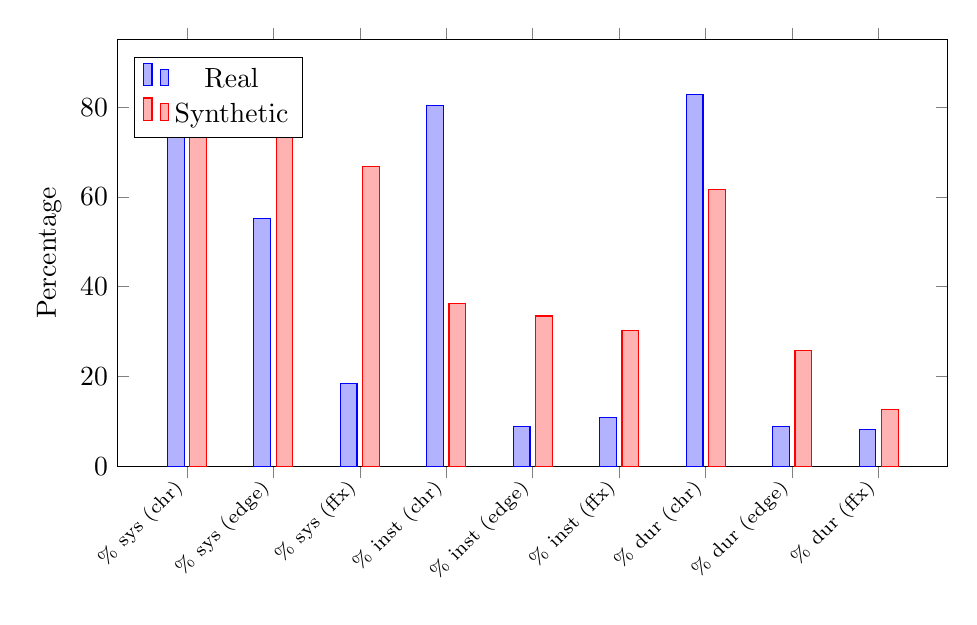
\begin{tikzpicture}
\begin{axis}[
    ybar,
    bar width=6pt,
    width=\linewidth,
    height=7cm,
    ylabel={Percentage},
    symbolic x coords={chrome-sys,edge-sys,firefox-sys,chrome-inst,edge-inst,firefox-inst,chrome-dur,edge-dur,firefox-dur},
    xtick=data,
    x tick label style={rotate=45, anchor=east, font=\scriptsize},
    legend style={at={(0.02,0.96)}, anchor=north west},
    ymin=0, ymax=95,
    xticklabels={\% sys (chr), \% sys (edge), \% sys (ffx), \% inst (chr), \% inst (edge), \% inst (ffx), \% dur (chr), \% dur (edge), \% dur (ffx)},
]
\addplot coordinates {
    (chrome-sys,82.05) (edge-sys,55.16) (firefox-sys,18.36)
    (chrome-inst,80.30) (edge-inst,8.91) (firefox-inst,10.79)
    (chrome-dur,82.89) (edge-dur,8.88) (firefox-dur,8.23)
};
\addplot coordinates {
    (chrome-sys,79.97) (edge-sys,73.90) (firefox-sys,66.78)
    (chrome-inst,36.24) (edge-inst,33.49) (firefox-inst,30.27)
    (chrome-dur,61.57) (edge-dur,25.73) (firefox-dur,12.70)
};
\legend{Real, Synthetic}
\end{axis}
\end{tikzpicture}
\caption{Browser usage metrics: percentage of systems, instances, and duration for chrome, edge, and firefox. The synthetic data preserves the relative ordering for duration but collapses the instance-level distribution toward uniformity ($\approx 33\%$ each), an artifact of the decomposition process assigning one row per \texttt{guid} per browser.}
\label{fig:browser-usage}
\end{figure}

The percent-systems metric is roughly preserved for chrome ($82.1\% \to 80.0\%$) but inflated for edge ($55.2\% \to 73.9\%$) and firefox ($18.4\% \to 66.8\%$). The percent-instances metric collapses to near-uniform ($\approx 33\%$ per browser) because the wide-table decomposition creates exactly one row per \texttt{guid} per browser, losing real instance-count variation.

\subsection{Continuous metric failure}

All queries involving continuous metrics (power, temperature, frequency, network bytes, memory utilization, battery duration) produce synthetic values near zero, with relative errors exceeding 99\%. Table~\ref{tab:continuous-failure} reports representative values for the five-way chassis join query and other continuous queries.

\begin{table}[H]
\centering
\begin{tabular}{lccc}
\toprule
\textbf{Metric} & \textbf{Real} & \textbf{Synthetic} & \textbf{Rel.\ error} \\
\midrule
avg\_psys\_rap\_watts & 4.42 & 0.002 & $> 99\%$ \\
avg\_pkg\_c0 (\%) & 37.4 & 0.022 & $> 99\%$ \\
avg\_freq\_mhz & 1{,}582 & 0.009 & $> 99\%$ \\
avg\_temp\_centigrade & 44.5 & 0.003 & $> 99\%$ \\
avg\_bytes\_received & $7.4 \times 10^{16}$ & 1.12 & $> 99\%$ \\
avg\_percentage\_used (\%) & 42.6 & 0.0 & $100\%$ \\
avg\_duration (battery, min) & 144 & 0.11 & $> 99\%$ \\
\bottomrule
\end{tabular}
\caption{Real vs.\ synthetic values for continuous metrics (notebook chassis type where applicable). All synthetic values are near zero.}
\label{tab:continuous-failure}
\end{table}

Figure~\ref{fig:ram-utilization} illustrates the failure on the RAM utilization histogram. Real data shows a clear inverse relationship between RAM capacity and utilization percentage. The synthetic data reports 0\% utilization across all capacities.

\begin{figure}[H]
\centering
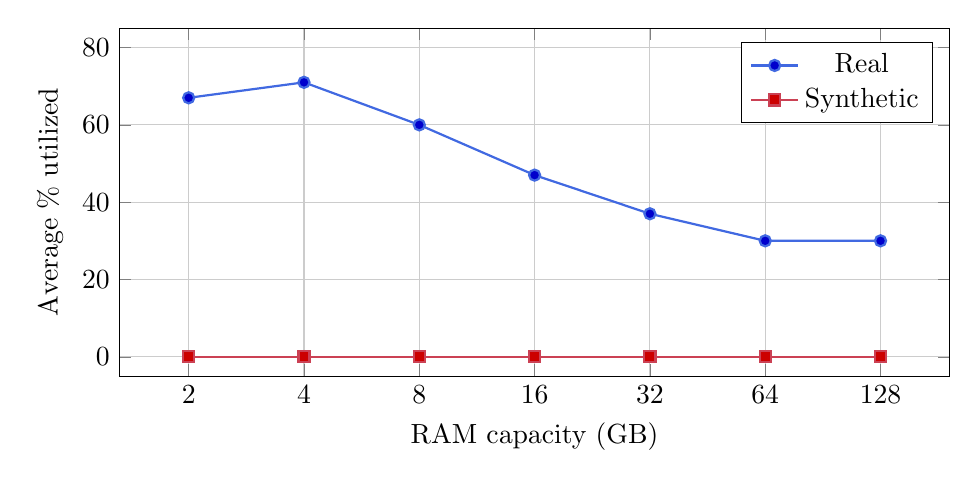
\begin{tikzpicture}
\begin{axis}[
    width=\linewidth,
    height=6cm,
    xlabel={RAM capacity (GB)},
    ylabel={Average \% utilized},
    xmode=log,
    log basis x=2,
    xtick={2,4,8,16,32,64,128},
    xticklabels={2,4,8,16,32,64,128},
    legend style={at={(0.98,0.96)}, anchor=north east},
    ymin=-5, ymax=85,
    grid=both,
    minor grid style={gray!20},
    major grid style={gray!40},
]
\addplot+[mark=*, thick, RoyalBlue] coordinates {
    (2,67) (4,71) (8,60) (16,47) (32,37) (64,30) (128,30)
};
\addlegendentry{Real}
\addplot+[mark=square*, thick, BrickRed] coordinates {
    (2,0) (4,0) (8,0) (16,0) (32,0) (64,0) (128,0)
};
\addlegendentry{Synthetic}
\end{axis}
\end{tikzpicture}
\caption{RAM utilization by capacity. Real data exhibits the expected inverse trend: devices with less RAM operate at higher utilization. The synthetic data produces 0\% utilization universally, as the memory columns in the wide table are zero for 93\% of \texttt{guid}s.}
\label{fig:ram-utilization}
\end{figure}

\subsection{Wide-table sparsity}

The continuous metric failure stems from extreme zero-inflation in the wide table. Most metric columns are nonzero for only a small fraction of the 1{,}000{,}000 \texttt{guid}s, because each event table covers a different subset of devices:

\begin{table}[H]
\centering
\begin{tabular}{lrr}
\toprule
\textbf{Metric source} & \textbf{Nonzero guids} & \textbf{Sparsity} \\
\midrule
PSYS RAP watts & 816 & 99.9\% \\
Average frequency & 613 & 99.9\% \\
Temperature & 622 & 99.9\% \\
C0 residency & 8{,}943 & 99.1\% \\
Network consumption & 37{,}224 & 96.3\% \\
Memory utilization & 69{,}552 & 93.0\% \\
\bottomrule
\end{tabular}
\caption{Nonzero coverage per metric in the wide table. The PSYS RAP, frequency, and temperature metrics have data for fewer than 0.1\% of \texttt{guid}s.}
\label{tab:sparsity}
\end{table}

The VAE optimizes mean squared error on these columns. When 93--99.9\% of values are zero, the loss-minimizing strategy is to generate near-zero values for all \texttt{guid}s. The KL divergence term further regularizes the latent space toward the standard normal, discouraging the model from learning a thin nonzero mode that accounts for less than 1\% of the data.

A secondary consequence is system count inflation. The five-way chassis join returns 104 real \texttt{guid}s (those with data in all five metric tables simultaneously). The synthetic data returns over 163{,}000 matches because the model generates small positive residuals for all \texttt{guid}s, causing the INNER JOIN to match far more rows than it should.

\newpage

\subsection{Four-method comparison}

Table~\ref{tab:method-comparison} summarizes the benchmark performance of all four synthesis methods. Both per-table methods (DP histogram and MST) pass 6 of 21 queries; the wide-table DP-VAE passes 1 of 8 evaluated queries. Private Evolution, which evaluates the same 8 wide-table queries, passes 2 of 8 (25.0\%).

\begin{table}[H]
\centering
\begin{tabular}{lccccc}
\toprule
\textbf{Method} & \textbf{Evaluated} & \textbf{Passed} & \textbf{Pass rate} & \textbf{Avg score} & \textbf{Median score} \\
\midrule
Wide-table DP-SGD & 8 & 1 & 12.5\% & 0.258 & 0.208 \\
Per-table DP-SGD & 21 & 6 & 28.6\% & 0.303 & 0.250 \\
MST baseline & 21 & 6 & 28.6\% & 0.328 & 0.250 \\
Private Evolution & 8 & 2 & 25.0\% & 0.150 & 0.000 \\
\bottomrule
\end{tabular}
\caption{Benchmark performance across synthesis methods. ``Passed'' counts queries with score $\geq 0.5$. The wide-table and PE methods evaluate only 8 queries because 13 require per-row columns absent from the wide-table representation.}
\label{tab:method-comparison}
\end{table}

The methods pass different subsets of queries. Table~\ref{tab:per-query-scores} reports per-query scores. All three non-PE methods correctly identify the most popular browser per country, while PE scores 0.000 on this query (13 of 15 overlapping countries correct, but only 15 of 51 real countries appear in the synthetic data). Both per-table methods pass the battery geographic summary and display vendor percentage queries. MST additionally passes the browser usage distribution and two application ranking queries, while per-table DP-SGD additionally passes the on/off sleep summary and RAM utilization histogram. PE passes the browser usage distribution (score 0.667, matching MST) and RAM utilization histogram (score 0.500, matching per-table DP-SGD). Neither per-table method passes any of the three userwait queries or the display connection type query.

% \begin{footnotesize}
\begin{longtable}{>{\raggedright\arraybackslash}p{0.33\linewidth}>{\raggedright\arraybackslash}p{0.10\linewidth}cccc}
\caption{Per-query scores for all four synthesis methods, color-coded by fidelity: \colorbox{scorehi}{\strut$\geq 0.5$} (pass), \colorbox{scoremid}{\strut$0.25$--$0.49$}, \colorbox{scorelo}{\strut$< 0.25$}, \colorbox{scorena}{\strut N/A}. Scores marked $\checkmark$ pass the 0.5 threshold.}
\label{tab:per-query-scores} \\
\toprule
\textbf{Query} & \textbf{Type} & \textbf{Wide} & \textbf{Per-table} & \textbf{MST} & \textbf{PE} \\
\midrule
\endfirsthead
\toprule
\textbf{Query} & \textbf{Type} & \textbf{Wide} & \textbf{Per-table} & \textbf{MST} & \textbf{PE} \\
\midrule
\endhead
\midrule
\multicolumn{6}{r}{\textit{Continued on next page}} \\
\endfoot
\bottomrule
\endlastfoot
\texttt{avg\_platform\_power\ldots chassis} & Agg+Join & \cellcolor{scorelo}0.167 & \cellcolor{scorelo}0.000 & \cellcolor{scorelo}0.000 & \cellcolor{scorelo}0.000 \\
\texttt{battery\_power\_on\ldots summary} & Geo/Demo & \cellcolor{scoremid}0.250 & \cellcolor{scorehi}1.000\,$\checkmark$ & \cellcolor{scorehi}0.500\,$\checkmark$ & \cellcolor{scorelo}0.000 \\
\texttt{Xeon\_network\_consumption} & Geo/Demo & \cellcolor{scoremid}0.250 & \cellcolor{scoremid}0.250 & \cellcolor{scoremid}0.250 & \cellcolor{scorelo}0.000 \\
\texttt{persona\_web\_cat\_usage\ldots} & Pivot & \cellcolor{scorelo}0.065 & \cellcolor{scoremid}0.419 & \cellcolor{scorelo}0.194 & \cellcolor{scorelo}0.032 \\
\texttt{pkg\_power\_by\_country} & Geo/Demo & \cellcolor{scoremid}0.333 & \cellcolor{scoremid}0.333 & \cellcolor{scoremid}0.333 & \cellcolor{scorelo}0.000 \\
\texttt{most\_popular\_browser\ldots country} & Top-$k$ & \cellcolor{scorehi}1.000\,$\checkmark$ & \cellcolor{scorehi}1.000\,$\checkmark$ & \cellcolor{scorehi}1.000\,$\checkmark$ & \cellcolor{scorelo}0.000 \\
\texttt{popular\_browsers\ldots percentage} & Histogram & \cellcolor{scorelo}0.000 & \cellcolor{scoremid}0.333 & \cellcolor{scorehi}0.667\,$\checkmark$ & \cellcolor{scorehi}0.667\,$\checkmark$ \\
\texttt{ram\_utilization\_histogram} & Histogram & \cellcolor{scorelo}0.000 & \cellcolor{scorehi}0.500\,$\checkmark$ & \cellcolor{scorelo}0.000 & \cellcolor{scorehi}0.500\,$\checkmark$ \\
\midrule
\texttt{battery\_on\_duration\ldots gen} & Geo/Demo & \cellcolor{scorena}--- & \cellcolor{scorelo}0.000 & \cellcolor{scorelo}0.000 & \cellcolor{scorena}--- \\
\texttt{display\_devices\ldots ac\_dc} & Agg+Join & \cellcolor{scorena}--- & \cellcolor{scorelo}0.000 & \cellcolor{scorelo}0.000 & \cellcolor{scorena}--- \\
\texttt{display\_devices\_vendors\ldots} & Agg+Join & \cellcolor{scorena}--- & \cellcolor{scorehi}1.000\,$\checkmark$ & \cellcolor{scorehi}1.000\,$\checkmark$ & \cellcolor{scorena}--- \\
\texttt{mods\_blockers\_by\_osname\ldots} & Agg+Join & \cellcolor{scorena}--- & \cellcolor{scoremid}0.250 & \cellcolor{scoremid}0.250 & \cellcolor{scorena}--- \\
\texttt{on\_off\_mods\_sleep\_summary\ldots} & Pivot & \cellcolor{scorena}--- & \cellcolor{scorehi}0.636\,$\checkmark$ & \cellcolor{scoremid}0.273 & \cellcolor{scorena}--- \\
\texttt{server\_exploration\_1} & Agg+Join & \cellcolor{scorena}--- & \cellcolor{scorelo}0.143 & \cellcolor{scoremid}0.429 & \cellcolor{scorena}--- \\
\texttt{top\_mods\_blocker\_types\ldots} & Agg+Join & \cellcolor{scorena}--- & \cellcolor{scorelo}0.000 & \cellcolor{scorelo}0.000 & \cellcolor{scorena}--- \\
\texttt{top\_10\_apps\ldots focal\_time} & Top-$k$ & \cellcolor{scorena}--- & \cellcolor{scorelo}0.000 & \cellcolor{scorelo}0.000 & \cellcolor{scorena}--- \\
\texttt{top\_10\_apps\ldots system\_count} & Top-$k$ & \cellcolor{scorena}--- & \cellcolor{scorelo}0.000 & \cellcolor{scorehi}1.000\,$\checkmark$ & \cellcolor{scorena}--- \\
\texttt{top\_10\_apps\ldots total\_detections} & Top-$k$ & \cellcolor{scorena}--- & \cellcolor{scorehi}0.500\,$\checkmark$ & \cellcolor{scorehi}1.000\,$\checkmark$ & \cellcolor{scorena}--- \\
\texttt{userwait\_top\_10\ldots processes} & Top-$k$ & \cellcolor{scorena}--- & \cellcolor{scorelo}0.000 & \cellcolor{scorelo}0.000 & \cellcolor{scorena}--- \\
\texttt{userwait\_top\_10\ldots ac\_dc} & Top-$k$ & \cellcolor{scorena}--- & \cellcolor{scorelo}0.000 & \cellcolor{scorelo}0.000 & \cellcolor{scorena}--- \\
\texttt{userwait\_top\_20\ldots unknown} & Top-$k$ & \cellcolor{scorena}--- & \cellcolor{scorelo}0.000 & \cellcolor{scorelo}0.000 & \cellcolor{scorena}--- \\
\end{longtable}
% \end{footnotesize}

Figure~\ref{fig:method-comparison} visualizes the overall pass rates and average scores.

\begin{figure}[H]
\centering
\begin{minipage}{0.48\linewidth}
\centering
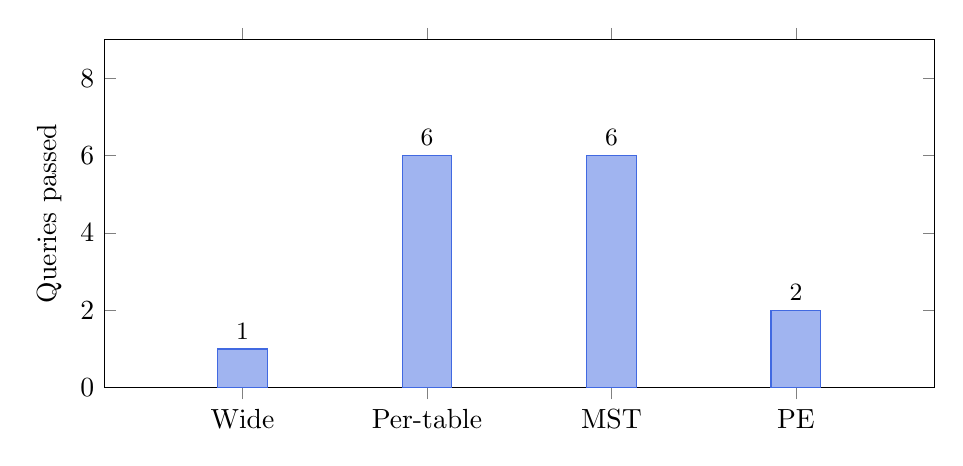
\begin{tikzpicture}
\begin{axis}[
    ybar,
    bar width=18pt,
    width=\linewidth,
    height=6cm,
    ylabel={Queries passed},
    symbolic x coords={Wide,Per-table,MST,PE},
    xtick=data,
    ymin=0, ymax=9,
    ytick={0,2,4,6,8},
    nodes near coords,
    every node near coord/.append style={font=\small},
    enlarge x limits=0.25,
]
\addplot[fill=RoyalBlue!50, draw=RoyalBlue] coordinates {(Wide,1) (Per-table,6) (MST,6) (PE,2)};
\end{axis}
\end{tikzpicture}
\end{minipage}
\hfill
\begin{minipage}{0.48\linewidth}
\centering
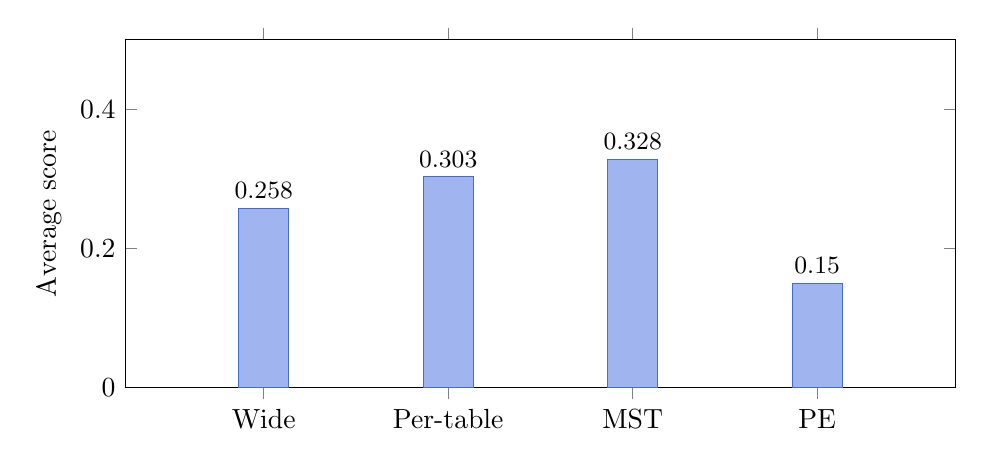
\begin{tikzpicture}
\begin{axis}[
    ybar,
    bar width=18pt,
    width=\linewidth,
    height=6cm,
    ylabel={Average score},
    symbolic x coords={Wide,Per-table,MST,PE},
    xtick=data,
    ymin=0, ymax=0.5,
    nodes near coords,
    every node near coord/.append style={font=\small, /pgf/number format/.cd, fixed, precision=3},
    enlarge x limits=0.25,
]
\addplot[fill=RoyalBlue!50, draw=RoyalBlue] coordinates {(Wide,0.258) (Per-table,0.303) (MST,0.328) (PE,0.150)};
\end{axis}
\end{tikzpicture}
\end{minipage}
\caption{Left: number of queries passing (score $\geq 0.5$) for each method. Right: average score across all evaluated queries. The per-table methods evaluate all 21 queries; the wide-table method evaluates 8.}
\label{fig:method-comparison}
\end{figure}

The per-query scores in Table~\ref{tab:per-query-scores}, color-coded by fidelity level, show that no method achieves high scores on aggregate queries involving continuous metrics, while categorical and ranking queries show more variation across methods.

Figure~\ref{fig:method-by-type} breaks down average scores by query type. The per-table methods achieve their strongest results on pivot and histogram queries, where the independent per-table approach avoids the zero-inflation that cripples the wide-table method. Aggregate queries involving multi-table joins remain the hardest category for all methods, with average scores below 0.3.

\begin{figure}[H]
\centering
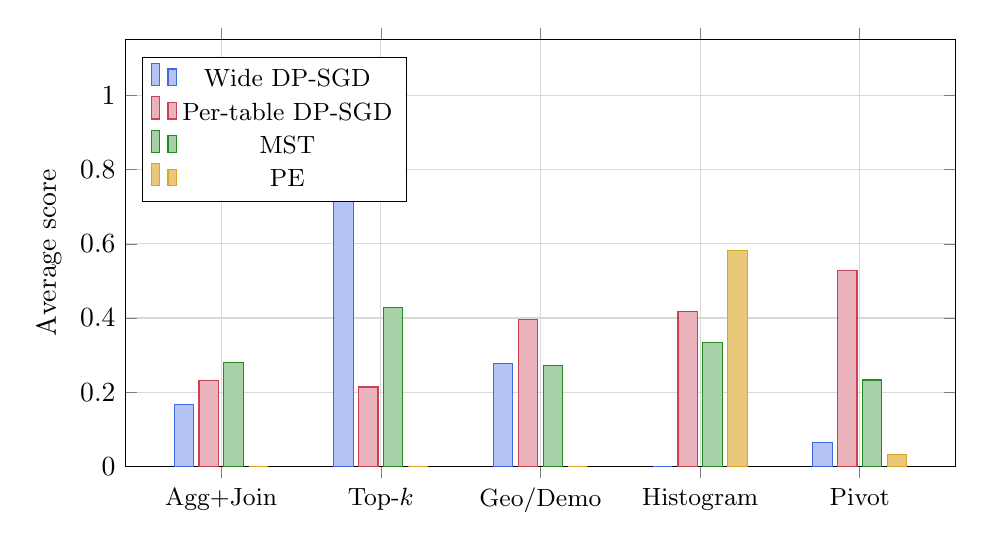
\begin{tikzpicture}
\begin{axis}[
    ybar,
    bar width=7pt,
    width=\linewidth,
    height=7cm,
    ylabel={Average score},
    symbolic x coords={Agg+Join,Top-$k$,Geo/Demo,Histogram,Pivot},
    xtick=data,
    ymin=0, ymax=1.15,
    ytick={0,0.2,0.4,0.6,0.8,1.0},
    legend style={at={(0.02,0.96)}, anchor=north west, font=\small},
    enlarge x limits=0.15,
    x tick label style={font=\small},
    grid=major,
    major grid style={gray!30},
]
\addplot[fill=RoyalBlue!40, draw=RoyalBlue] coordinates {
    (Agg+Join,0.167) (Top-$k$,1.000) (Geo/Demo,0.278) (Histogram,0.000) (Pivot,0.065)
};
\addplot[fill=BrickRed!40, draw=BrickRed] coordinates {
    (Agg+Join,0.232) (Top-$k$,0.214) (Geo/Demo,0.396) (Histogram,0.417) (Pivot,0.528)
};
\addplot[fill=ForestGreen!40, draw=ForestGreen] coordinates {
    (Agg+Join,0.280) (Top-$k$,0.429) (Geo/Demo,0.271) (Histogram,0.333) (Pivot,0.233)
};
\addplot[fill=Goldenrod!60, draw=Goldenrod] coordinates {
    (Agg+Join,0.000) (Top-$k$,0.000) (Geo/Demo,0.000) (Histogram,0.583) (Pivot,0.032)
};
\legend{Wide DP-SGD, Per-table DP-SGD, MST, PE}
\end{axis}
\end{tikzpicture}
\caption{Average query score by query type across synthesis methods. The wide-table method evaluates 1--3 queries per type (vs.\ 2--7 for per-table methods), so its per-type averages have higher variance.}
\label{fig:method-by-type}
\end{figure}

\subsection{Method complementarity}

Per-table DP-SGD and MST pass different subsets of queries, revealing complementary strengths tied to each algorithm's treatment of continuous versus categorical data.

Per-table DP-SGD excels on queries requiring accurate continuous values. The battery geographic summary passes all four metrics (Jaccard = 0.79, system count RE = 0.12, power-on count RE = 0.14, duration RE = 0.24). The on/off sleep summary passes 7 of 11 metrics, with on-time RE = 0.13, off-time RE = 0.15, sleep-time RE = 0.04, and total-time RE = 0.07. The DP histogram synthesis preserves the shape of continuous distributions because it samples from the noisy empirical distribution directly, and the Laplace noise on bin counts is small relative to the signal when the table has tens of thousands of rows.

MST excels on queries requiring accurate rankings. The top-10 applications by system count achieves a perfect score (Jaccard = 0.41, Spearman $\rho$ = 1.00), while per-table DP-SGD scores 0.00 on the same query (Jaccard = 0.13, $\rho$ = $-0.05$). Similarly, top-10 by total detections: MST achieves $\rho$ = 0.71 versus per-table's 0.11. MST preserves rankings because it captures pairwise marginals between the application name and the count column, maintaining relative ordering even when absolute values are noisy.

Both methods fail on the three userwait queries (score 0.00 each). The userwait table contains 175M rows across 38{,}142 \texttt{guid}s with process names, wait types, and AC/DC power states. The per-table approach generates the correct table structure but cannot reproduce the long-tailed distribution of process-specific wait times. MST bins the continuous wait duration into marginals, losing the per-process ranking that the queries test.

The 5-way chassis join query (\texttt{avg\_platform\_power\_c0\_freq\_temp\_by\_chassis}) fails for both per-table methods (score 0.00) because it requires correlations across five independently synthesized tables. The wide-table approach scores 0.17 on this query, the only method that produces any correct values, because it preserves the joint distribution (though the values are near-zero due to sparsity).

MST produces dramatically different continuous values from per-table DP-SGD on the same queries. On the on/off sleep summary, MST reports avg\_on\_time RE = 40.2 and avg\_off\_time RE = 45.1 (the synthesized values are 40$\times$ too large), while per-table DP-SGD reports RE = 0.13 and 0.15 respectively. On the battery geographic summary, MST's avg\_duration RE = 28.2 versus per-table's 0.24. This difference arises because MST discretizes all columns into marginal bins, and the bin midpoints can be far from the true conditional means when the distribution is skewed.

\subsection{Private Evolution}

PE completes generation of 150{,}000 candidates via the OpenAI Batch API (gpt-5-nano), followed by the DP nearest-neighbor histogram ($\sigma \approx 1.08$) and rank-based selection of 50{,}000 records. Total wall-clock time is 59 minutes, of which the histogram computation accounts for the majority. The final privacy expenditure is $\varepsilon = 4.0$ at $\delta = 10^{-5}$.

PE passes 2 of 8 evaluated queries (25.0\%), with an average score of 0.150. The two passing queries are the browser usage distribution (score 0.667) and the RAM utilization histogram (score 0.500). These are the same query types where the DP nearest-neighbor histogram can correct for the foundation model's distributional biases: the histogram selects candidates whose browser and RAM distributions best match the real data, even though the raw LLM output deviates substantially.

All aggregate and geographic queries score 0.000. The 5-way chassis join, network consumption, battery summary, and power-by-country queries all fail because the selected synthetic records contain near-zero values for continuous metrics. The browser ranking query also scores 0.000. PE generates only 15 of 51 real countries (vs.\ 50 for the wide-table DP-VAE), and achieves 13 correct among those 15, because the foundation model's categorical priors concentrate on a narrow set of countries and distort the joint distribution between country and browser preference. The persona web category pivot scores 0.032 (1 of 31 metrics passing).

Categorical distributions in the PE output show systematic deviations from the real data. The model over-represents Win11 (77.8\% vs.\ 10.4\% real) and under-represents Win10 (9.2\% vs.\ 86.2\% real), reflecting the foundation model's training data distribution rather than the DCA telemetry distribution. The model also generates hallucinated categorical values not present in the real data: 132 extra \texttt{chassistype} values (including misspellings like ``Noteboook'', ``DeskTop'', ``NoteBook''), 33 extra countries (leading-whitespace variants like `` Brazil''), and 15 extra OS values (including ``WinServer'', ``n/a''). These hallucinated values always score as maximum mismatch in the workload-aware distance function, wasting a portion of the generation budget.

Numeric columns exhibit the same sparsity problem as DP-SGD. The foundation model generates near-zero values for sparse metrics: network bytes, memory utilization, battery duration, and all hardware metrics have $< 1\%$ nonzero rates in the synthetic data (vs.\ 2--7\% in real data). The model has learned that most fields are zero (the prompt describes the sparsity structure), but it generates too few nonzero records relative to the real distribution.

\section{Discussion}

The four-method comparison provides answers to several of our research questions.

Research question (1), which method achieves higher benchmark scores, has a nuanced answer. Per-table DP-SGD and MST both pass 6 of 21 queries (28.6\%), with MST achieving a slightly higher average score (0.328 vs.\ 0.303). The wide-table DP-VAE passes 1 of 8 evaluated queries (12.5\%). PE passes 2 of 8 (25.0\%), outperforming the wide-table DP-VAE on the same query set but with a lower average score (0.150 vs.\ 0.258). No method comes close to passing all queries. The two per-table methods pass different query subsets: per-table DP-SGD passes the on/off sleep summary (score 0.64) and RAM histogram (0.50), while MST passes browser usage distribution (0.67) and two application ranking queries (1.00 each). PE's two passing queries (browser usage distribution at 0.667 and RAM histogram at 0.500) overlap with the per-table methods, indicating that the DP histogram selection can correct distributional biases in the LLM output for histogram-type queries. This complementarity reflects fundamental algorithmic differences. DP histogram synthesis preserves continuous distributions by sampling from noisy bin counts, yielding low relative error on time-based metrics (on-time RE = 0.13, sleep-time RE = 0.04). MST preserves pairwise marginals between categorical keys and count columns, maintaining rankings (Spearman $\rho$ = 1.00 on application system counts) even when absolute values are distorted. Neither algorithm achieves both properties simultaneously.

Research question (2), whether error compounds across multi-table joins, receives a clear affirmative. The 5-way chassis join query requires data from five independently synthesized tables. Both per-table methods score 0.00 because the synthetic tables share no correlated \texttt{guid}s; the inner join produces empty results (per-table DP-SGD) or random associations (MST). The wide-table DP-VAE scores 0.17 on this query, the only method that preserves any cross-table structure, but the values are near-zero due to sparsity. The server exploration query (a 2-way join) similarly suffers: both per-table methods overcount matching rows by 5--7$\times$ and report network byte values with RE $\approx 1.0$, because the independently synthesized network and sysinfo tables produce spurious \texttt{guid} overlaps.

Research question (3), minority class preservation, is partially addressed. The browser ranking query demonstrates that all methods preserve dominant categorical associations: per-table DP-SGD achieves 47 of 50 correct top browsers per country, and the wide-table DP-VAE achieves 42 of 50. For rare categories, per-table DP-SGD inflates minority chassis types (``Intel NUC/STK'' at 8.4\% synthetic vs.\ 2.0\% real) due to the top-50 binning and uniform noise in DP-SGD, while MST underrepresents them (generating too few entries for rare combinations). Both methods underperform on queries involving rare process names or application-specific rankings.

Research question (4), classifier comparability, remains unaddressed. The benchmark queries are analytical (aggregate statistics, rankings, distributions), not predictive, so training downstream classifiers on the synthetic data was not a natural fit for this evaluation framework. A direct comparison would require defining a classification task on the DCA data (e.g., predicting chassis type from usage patterns), training models on real versus synthetic data, and comparing test accuracy. We defer this to future work.

Research question (5), wall-clock time, shows clear differences. The wide-table DP-VAE trains in 360 minutes on CPU (20 epochs, 1M rows, 307 features). Per-table synthesis completes in approximately 90 minutes total (two VAEs at $\sim$30 minutes each for sysinfo and cpu\_metadata, plus histogram synthesis for 17 smaller tables). MST runs in under 10 minutes per table using the \texttt{mst} library. PE completes in 59 minutes total: the OpenAI Batch API generates 150{,}000 candidate records (7{,}500 batch calls at approximately \$18--37), and the DP nearest-neighbor histogram over 1{,}000{,}000 real $\times$ 150{,}000 synthetic records accounts for the remaining computation.

The PE results confirm that foundation models import their own distributional priors rather than learning the target distribution (Win11 at 77.8\% vs.\ 10.4\% real). The DP nearest-neighbor histogram partially corrects these biases for histogram-type queries (PE matches MST on browser usage at 0.667 and outperforms the wide-table DP-VAE on RAM utilization at 0.500 vs.\ 0.000), but cannot compensate for the near-total absence of nonzero continuous metrics in the LLM output. The hallucinated categorical values further reduce effective sample size by generating records that cannot match any real data point in the nearest-neighbor histogram. This aligns with \citeauthor{swanberg2025apiaccessllmsuseful}'s finding that LLMs capture 1-way marginals reasonably but are inaccurate on $k$-way marginals.

Several mitigation strategies warrant investigation:

\begin{itemize}
    \item A two-stage model in which a Bernoulli model predicts zero vs.\ nonzero per column, followed by a conditional model for nonzero values only.
    \item Relational DP synthesis methods that handle multi-table structure directly, eliminating the zero-inflation problem while preserving cross-table correlations.
    \item Method ensembling: using per-table DP-SGD for queries requiring continuous accuracy and MST for queries requiring ranking preservation, selecting per query type.
    \item Post-processing the synthetic data with mode patching and constraint enforcement, as proposed by recent work on model-agnostic DP post-processing.
\end{itemize}

\subsection{Sensitivity to evaluation thresholds}

Figure~\ref{fig:sensitivity} reports how pass rates change as the relative error, total variation, and Spearman $\rho$ thresholds vary. The analysis confirms that our findings are not artifacts of a particular threshold choice.

The relative error threshold has the largest effect. Per-table DP-SGD's pass rate increases from 14.3\% at RE $\leq 0.05$ to 57.1\% at RE $\leq 1.0$, indicating many queries produce synthetic values in the right order of magnitude but outside the strict 25\% tolerance. MST is more robust to strict thresholds: it starts at 23.8\% at RE $\leq 0.05$ (compared to 14.3\% for per-table), reflecting its strength on categorical distributions where exact values are less important than distributional shape. The wide-table method is flat at 12.5\% until RE $\leq 1.0$, at which point it jumps to 75\%, confirming that the continuous metric failure is total (relative errors exceed 99\%) rather than marginal.

Total variation and Spearman $\rho$ thresholds have minimal effect on pass rates across all methods. TV sensitivity is limited because the distribution queries either match closely (TV $< 0.10$) or fail badly (TV $> 0.5$), with few queries in the boundary region. Rank correlation sensitivity is limited because MST achieves perfect $\rho = 1.0$ on its passing ranking queries while both methods score near zero on failing ones, leaving no queries sensitive to the threshold.

\begin{figure}[H]
\centering
\begin{minipage}{0.32\linewidth}
\centering
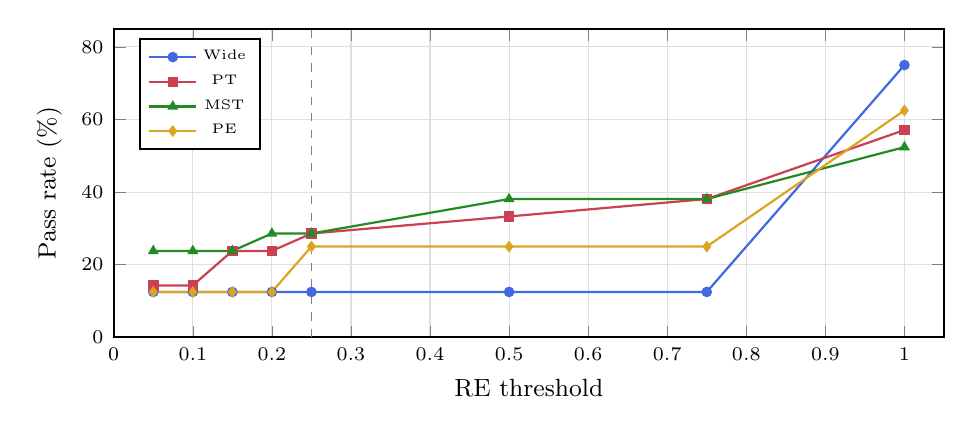
\begin{tikzpicture}
\begin{axis}[
    width=\linewidth,
    height=5.5cm,
    xlabel={\small RE threshold},
    ylabel={\small Pass rate (\%)},
    xmin=0, xmax=1.05,
    ymin=0, ymax=85,
    legend style={at={(0.03,0.97)}, anchor=north west, font=\tiny},
    grid=major,
    major grid style={gray!25},
    mark size=1.5pt,
    line width=0.8pt,
    tick label style={font=\scriptsize},
]
\addplot[RoyalBlue, mark=*] coordinates {
    (0.05,12.5) (0.10,12.5) (0.15,12.5) (0.20,12.5)
    (0.25,12.5) (0.50,12.5) (0.75,12.5) (1.00,75.0)
};
\addplot[BrickRed, mark=square*] coordinates {
    (0.05,14.3) (0.10,14.3) (0.15,23.8) (0.20,23.8)
    (0.25,28.6) (0.50,33.3) (0.75,38.1) (1.00,57.1)
};
\addplot[ForestGreen, mark=triangle*] coordinates {
    (0.05,23.8) (0.10,23.8) (0.15,23.8) (0.20,28.6)
    (0.25,28.6) (0.50,38.1) (0.75,38.1) (1.00,52.4)
};
\addplot[Goldenrod, mark=diamond*] coordinates {
    (0.05,12.5) (0.10,12.5) (0.15,12.5) (0.20,12.5)
    (0.25,25.0) (0.50,25.0) (0.75,25.0) (1.00,62.5)
};
\draw[gray, dashed, thin] (axis cs:0.25,0) -- (axis cs:0.25,85);
\legend{Wide, PT, MST, PE}
\end{axis}
\end{tikzpicture}
\end{minipage}
\hfill
\begin{minipage}{0.32\linewidth}
\centering
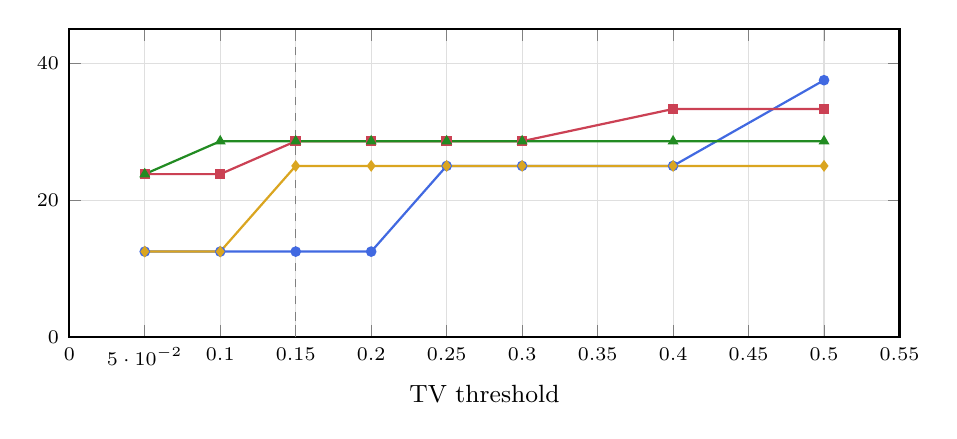
\begin{tikzpicture}
\begin{axis}[
    width=\linewidth,
    height=5.5cm,
    xlabel={\small TV threshold},
    xmin=0, xmax=0.55,
    ymin=0, ymax=45,
    grid=major,
    major grid style={gray!25},
    mark size=1.5pt,
    line width=0.8pt,
    tick label style={font=\scriptsize},
]
\addplot[RoyalBlue, mark=*] coordinates {
    (0.05,12.5) (0.10,12.5) (0.15,12.5) (0.20,12.5)
    (0.25,25.0) (0.30,25.0) (0.40,25.0) (0.50,37.5)
};
\addplot[BrickRed, mark=square*] coordinates {
    (0.05,23.8) (0.10,23.8) (0.15,28.6) (0.20,28.6)
    (0.25,28.6) (0.30,28.6) (0.40,33.3) (0.50,33.3)
};
\addplot[ForestGreen, mark=triangle*] coordinates {
    (0.05,23.8) (0.10,28.6) (0.15,28.6) (0.20,28.6)
    (0.25,28.6) (0.30,28.6) (0.40,28.6) (0.50,28.6)
};
\addplot[Goldenrod, mark=diamond*] coordinates {
    (0.05,12.5) (0.10,12.5) (0.15,25.0) (0.20,25.0)
    (0.25,25.0) (0.30,25.0) (0.40,25.0) (0.50,25.0)
};
\draw[gray, dashed, thin] (axis cs:0.15,0) -- (axis cs:0.15,45);
\end{axis}
\end{tikzpicture}
\end{minipage}
\hfill
\begin{minipage}{0.32\linewidth}
\centering
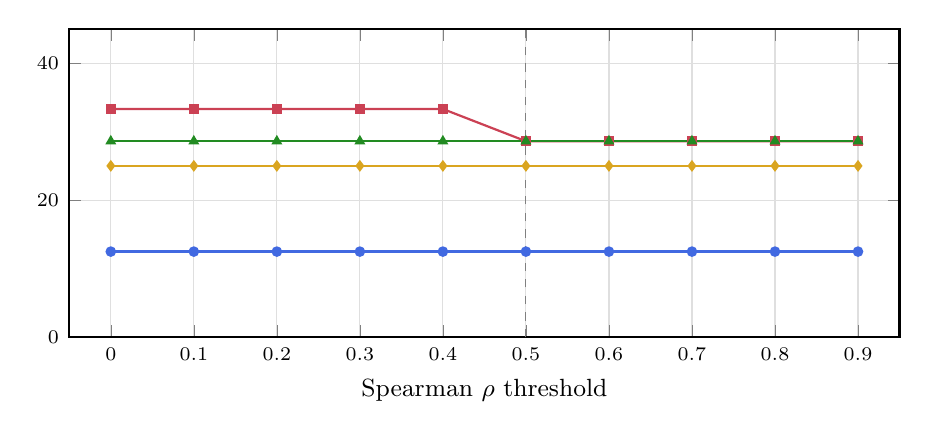
\begin{tikzpicture}
\begin{axis}[
    width=\linewidth,
    height=5.5cm,
    xlabel={\small Spearman $\rho$ threshold},
    xmin=-0.05, xmax=0.95,
    ymin=0, ymax=45,
    grid=major,
    major grid style={gray!25},
    mark size=1.5pt,
    line width=0.8pt,
    tick label style={font=\scriptsize},
]
\addplot[RoyalBlue, mark=*] coordinates {
    (0.0,12.5) (0.1,12.5) (0.2,12.5) (0.3,12.5) (0.4,12.5)
    (0.5,12.5) (0.6,12.5) (0.7,12.5) (0.8,12.5) (0.9,12.5)
};
\addplot[BrickRed, mark=square*] coordinates {
    (0.0,33.3) (0.1,33.3) (0.2,33.3) (0.3,33.3) (0.4,33.3)
    (0.5,28.6) (0.6,28.6) (0.7,28.6) (0.8,28.6) (0.9,28.6)
};
\addplot[ForestGreen, mark=triangle*] coordinates {
    (0.0,28.6) (0.1,28.6) (0.2,28.6) (0.3,28.6) (0.4,28.6)
    (0.5,28.6) (0.6,28.6) (0.7,28.6) (0.8,28.6) (0.9,28.6)
};
\addplot[Goldenrod, mark=diamond*] coordinates {
    (0.0,25.0) (0.1,25.0) (0.2,25.0) (0.3,25.0) (0.4,25.0)
    (0.5,25.0) (0.6,25.0) (0.7,25.0) (0.8,25.0) (0.9,25.0)
};
\draw[gray, dashed, thin] (axis cs:0.5,0) -- (axis cs:0.5,45);
\end{axis}
\end{tikzpicture}
\end{minipage}
\caption{Pass rate sensitivity to evaluation thresholds. Left: relative error threshold (TV = 0.15, $\rho$ = 0.5 fixed). Center: total variation threshold (RE = 0.25, $\rho$ = 0.5 fixed). Right: Spearman $\rho$ threshold (RE = 0.25, TV = 0.15 fixed). Dashed gray lines indicate the default thresholds.}
\label{fig:sensitivity}
\end{figure}

\section{Conclusion}

We presented an evaluation framework for differentially private synthetic data generation on Intel's DCA telemetry corpus, implementing four synthesis approaches: a wide-table DP-VAE trained with DP-SGD, per-table DP histogram synthesis, MST marginal-based synthesis, and Private Evolution via foundation model APIs.

All four methods have completed evaluation against the 21-query benchmark. Per-table DP-SGD and MST each pass 6 of 21 queries (28.6\% pass rate), passing different subsets that reflect their algorithmic strengths: DP histogram synthesis preserves continuous distributions (on-time RE = 0.13) while MST preserves rankings (Spearman $\rho$ = 1.00 on application counts). The wide-table DP-VAE passes 1 of 8 evaluated queries (12.5\%), with all continuous metrics near zero due to extreme sparsity in the wide-table representation. PE passes 2 of 8 (25.0\%), outperforming the wide-table DP-VAE in pass count but with a lower average score (0.150 vs.\ 0.258). PE's two passing queries (browser usage distribution and RAM utilization histogram) are histogram-type queries where the DP nearest-neighbor selection can correct the foundation model's distributional biases.

Two structural findings emerge. First, wide-table sparsity, not the choice of synthesis algorithm, is the dominant failure mode. The wide table has 93--99.9\% zero values in metric columns, and both the VAE and the foundation model collapse these to their mode. Second, per-table independence destroys cross-table correlations: the 5-way chassis join produces empty or random results under both per-table methods, while the wide-table approaches (DP-VAE and PE) at least preserve some cross-table structure.

PE confirms the negative result of \citet{swanberg2025apiaccessllmsuseful}: API access to foundation models does not improve DP tabular synthesis beyond established baselines on the DCA corpus. The foundation model imports its own distributional priors (Win11 at 77.8\% vs.\ 10.4\% real), hallucinates categorical values outside the real vocabulary, and generates near-zero continuous metrics. The DP histogram partially corrects distributional queries but cannot compensate for the absence of signal in aggregate and geographic queries.

These results point toward relational DP synthesis as the most promising direction: methods that handle multi-table structure directly could eliminate zero-inflation while preserving cross-table correlations. A secondary direction is method ensembling, selecting per-table DP-SGD for continuous-valued queries and MST for ranking queries, capitalizing on their complementary strengths.

\newpage

\makereference

\nocite{*}
\bibliography{reference}
\bibliographystyle{style/dsc180bibstyle}

\newpage
\appendix

\section{Project proposal}

The following is reproduced from the Q2 project proposal submitted in Fall 2025.

\subsection{Problem statement}

Organizations routinely collect detailed telemetry from their products that drive critical business decisions. The same granularity that makes telemetry valuable also makes it sensitive. Differential privacy (DP) provides a rigorous mathematical framework for releasing data while bounding the influence of any individual record. Two paradigms have emerged for generating differentially private synthetic data. Training-based methods (DP-SGD) inject noise during model optimization, while training-free methods (Private Evolution) achieve privacy through black-box API access to foundation models.

We implement and compare both approaches on Intel's Driver and Client Applications (DCA) telemetry corpus, evaluating against a benchmark of analytical SQL queries representative of production business intelligence workloads. Under matched privacy budgets ($\varepsilon = 4.0$, $\delta = 10^{-5}$), we assess query fidelity, statistical preservation, and computational cost to determine whether training-free methods can match training-based approaches on real multi-table relational data.

\subsection{Data}

The DCA telemetry corpus comprises approximately 30 interrelated tables organized around a globally unique client identifier (\texttt{guid}). Tables span system metadata, power and thermal instrumentation, battery usage, application behavior, web browsing, network consumption, and display devices. We construct 19 reporting tables from the raw data, each aggregated to the \texttt{guid} level, and define a benchmark of 21 feasible SQL queries covering aggregate statistics with joins, ranked top-$k$ lists, geographic and demographic breakdowns, histograms, and complex multi-way pivots.

\subsection{Methods}

For training-based synthesis, we implement a differentially private variational autoencoder (DP-VAE) using PyTorch and the Opacus library, with privacy guarantees via DP-SGD (per-sample gradient clipping and calibrated noise injection). For training-free synthesis, we implement Private Evolution using black-box API access to foundation models, achieving privacy through differentially private nearest-neighbor histograms. Both methods are evaluated under matched privacy budgets on the 21-query SQL benchmark.

\subsection{Research questions}

\begin{enumerate}
    \item Under matched $(\varepsilon, \delta)$, which method achieves higher scores on the SQL query benchmark?
    \item Does error compound across multi-table joins?
    \item Which method better preserves minority class frequencies?
    \item Do classifiers trained on synthetic data achieve comparable accuracy to those trained on real data?
    \item What are the wall-clock time and resource requirements for each method?
\end{enumerate}

\subsection{Expected outputs}

\begin{enumerate}
    \item Technical report with implementation details, privacy analysis, and query-by-query benchmark results.
    \item SQL benchmark suite (21 queries with natural language specifications, SQL code, and evaluation scripts).
    \item Two differentially private synthetic DCA datasets (one DP-SGD, one PE) with documented privacy guarantees.
    \item Project website with visualizations and deployment guidelines.
    \item Open-source implementations for preprocessing, training, generation, and evaluation.
\end{enumerate}

\newpage

\section{Contributions}

\noindent Jason Tran: Built the 19 reporting tables from raw telemetry data via DuckDB aggregation scripts. Designed and implemented the wide-table construction, DP-VAE architecture, DP-SGD training pipeline, synthetic data generation, and benchmark evaluation framework. Wrote the report.

\medskip
\noindent Mehak Kapur: Ran and validated DuckDB queries to ingest the Parquet datasets. Helped construct the unified wide training table. Implemented and executed the DP-SGD VAE pipeline to generate synthetic data. Produced evaluation outputs and visualizations comparing real versus synthetic distributions. Wrote the report.

\medskip
\noindent Hana Tjendrawasi: Ran and validated DuckDB queries to ingest the Parquet datasets. Helped construct the unified wide training table by aligning schemas across sources. Supported the DP-SGD workflow through preprocessing and experiment setup. Assisted with reviewing evaluation metrics and results. Wrote the report.

\medskip
\noindent Phuc Tran: Exploratory data analysis on raw telemetry tables. Schema verification and column mapping between raw and reporting tables.

\end{document}
